% !TEX root = DesignDocument.tex


\chapter{Prototypes}

This chapter is for recording each prototype developed.  It is a historical record of what you accomplished in 464/465.   This should be organized according to Sprints.  It should have the basic description of the sprint deliverable and what was accomplished.  Screen shots, photos, captures from video, etc should be used.  

\section{Sprint 1 Prototype}
\subsection{Deliverable}
Rough draft of main page. See Figure~\ref{prototype_S1_main}.

\begin{figure}[tbh]
\begin{center}
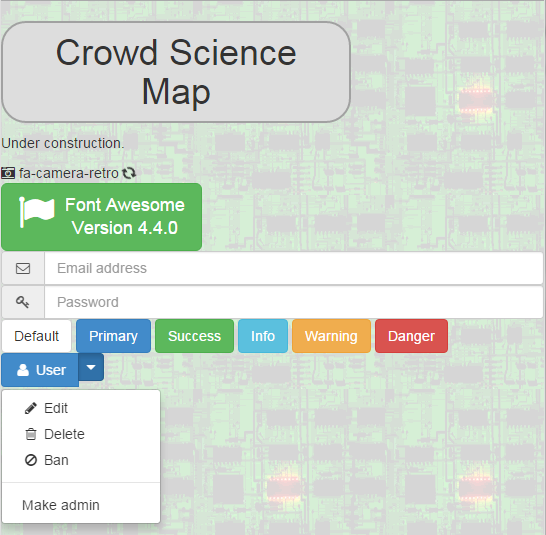
\includegraphics[width=0.75\textwidth]{./figures/prototype_S1_main.png}
\end{center}
\caption{Crowd Science Main Page Prototype as of Sprint 1\label{prototype_S1_main}}
\end{figure}

\subsection{Backlog}
The backlog completed for this sprint was initial documentation, primarily including the requirements section of the design document; an analysis of the work done in the previous project, the Landscape Change Mapper; and creating a rough draft of the Crowd Science Mapper website.
\subsection{Success/Fail}
This sprint was a success, overall. No major issues arose.

\section{Sprint 2 Prototype}
\subsection{Deliverable}
Updated main page, added login and register features. See Figure~\ref{prototype_S2_main}, Figure~\ref{prototype_S2_login}, and Figure~\ref{prototype_S2_register}.

\begin{figure}[tbh]
\begin{center}
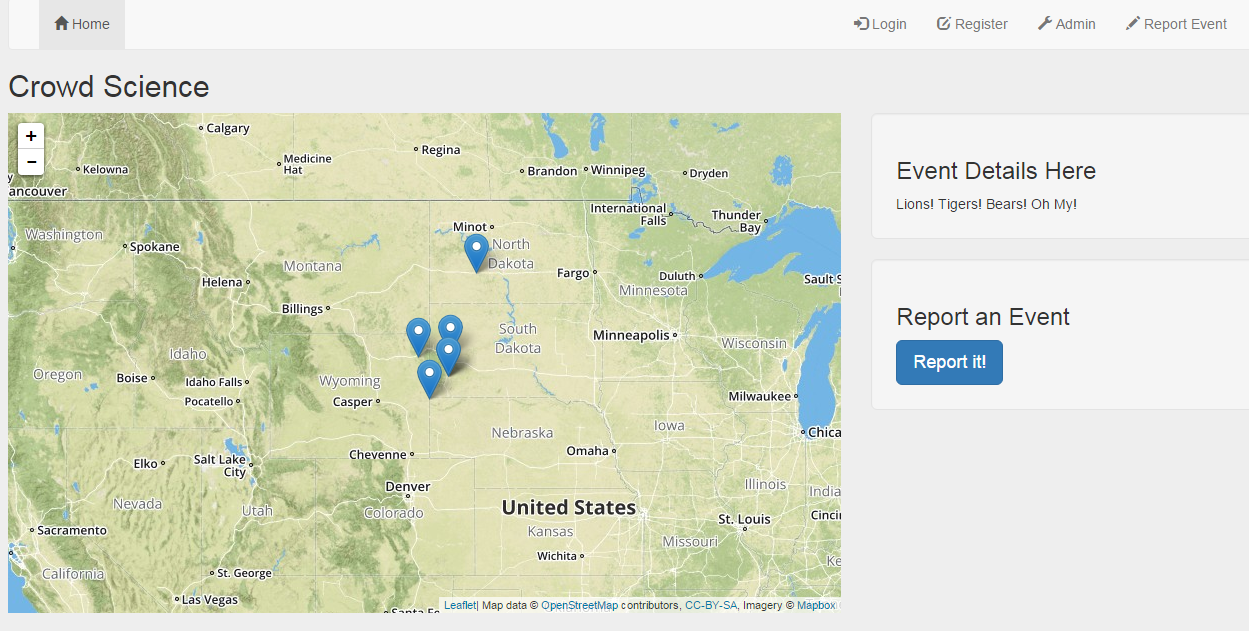
\includegraphics[width=0.75\textwidth]{./figures/prototype_S2_main.png}
\end{center}
\caption{Crowd Science Main Page Prototype as of Sprint 2\label{prototype_S2_main}}
\end{figure}

\begin{figure}[tbh]
\begin{center}
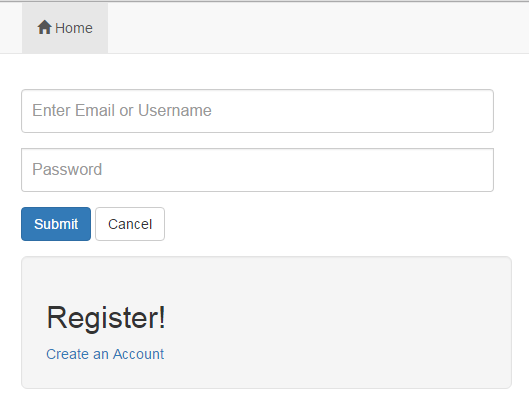
\includegraphics[width=0.75\textwidth]{./figures/prototype_S2_login.png}
\end{center}
\caption{Crowd Science Login Page Prototype as of Sprint 2\label{prototype_S2_login}}
\end{figure}

\begin{figure}[tbh]
\begin{center}
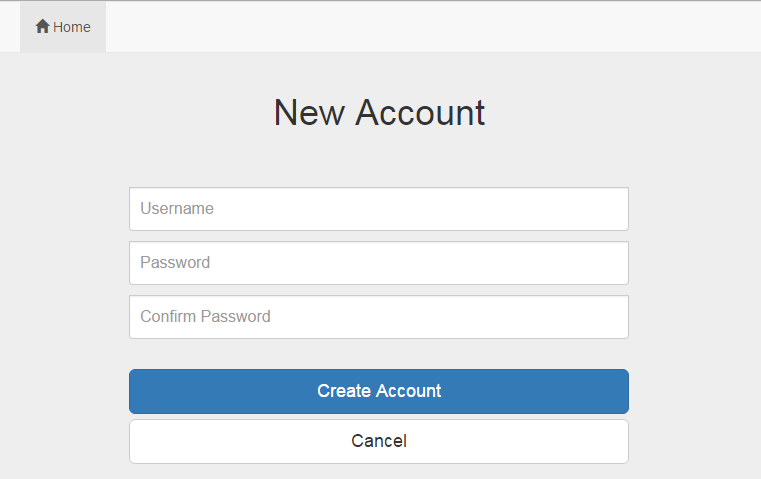
\includegraphics[width=0.75\textwidth]{./figures/prototype_S2_register.png}
\end{center}
\caption{Crowd Science Register Page Prototype as of Sprint 2\label{prototype_S2_register}}
\end{figure}


\subsection{Backlog}
The backlog completed for this sprint was a completed analysis of original project, the LCM; expansion on the original draft to include login and register page layouts; transporting code from LCM project for login and register pages and adapting the code for our project; and more work on the requirements, project, and mission/elevator sections.
\subsection{Success/Fail}
This sprint was a success, overall. No major issues arose.

\section{Sprint 3 Prototype}
\subsection{Deliverable}
There were no changes to the deliverable of Sprint 2.
\subsection{Backlog}
The backlog completed for this sprint was work on the requirements section and overview section. 
\subsection{Success/Fail}
This sprint was a roaring failure, overall. Following the client presentation on 10/27/2015, Jiasong entirely ceased contributing to the project and attending team meetings. The features planned to be added to the prototype, submitting a report and viewing a list of reports; were not added to the prototype.

\section{Sprint 4 Prototype}
\subsection{Deliverable}
Added event set selection to main page, added feilds to register page. See Figure~\ref{prototype_S4_main}, Figure~\ref{prototype_S4_selectbox}, Figure~\ref{prototype_S4_login} , and Figure~\ref{prototype_S4_register}.

\begin{figure}[tbh]
\begin{center}
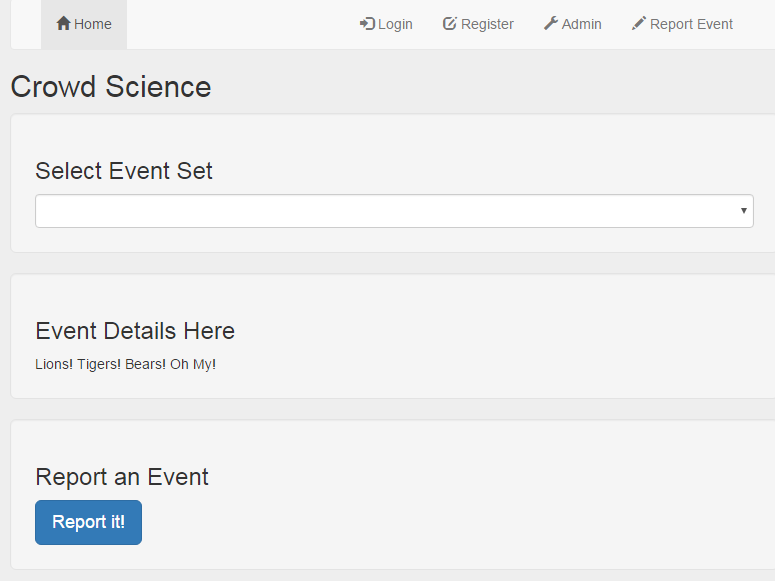
\includegraphics[width=0.75\textwidth]{./figures/prototype_S4_main.png}
\end{center}
\caption{Crowd Science Main Page Prototype as of Sprint 4\label{prototype_S4_main}}
\end{figure}

\begin{figure}[tbh]
\begin{center}
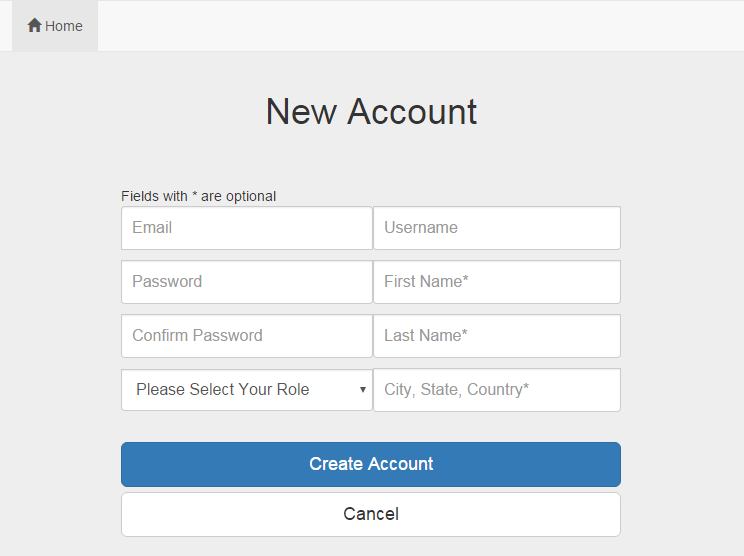
\includegraphics[width=0.75\textwidth]{./figures/prototype_S4_register.png}
\end{center}
\caption{Crowd Science Register Page Prototype as of Sprint 4\label{prototype_S4_register}}
\end{figure}

\begin{figure}[tbh]
\begin{center}
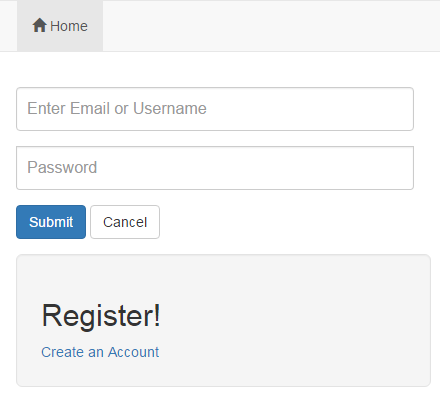
\includegraphics[width=0.75\textwidth]{./figures/prototype_S4_login.png}
\end{center}
\caption{Crowd Science Login Page Prototype as of Sprint 4\label{prototype_S4_login}}
\end{figure}

\begin{figure}[tbh]
\begin{center}
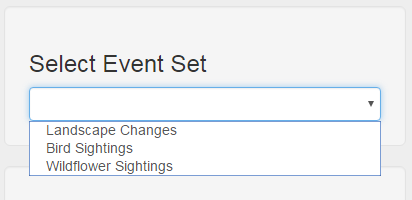
\includegraphics[width=0.75\textwidth]{./figures/prototype_S4_selectbox.png}
\end{center}
\caption{Crowd Science Event Set Selection Prototype as of Sprint 4\label{prototype_S4_selectbox}}
\end{figure}

\subsection{Backlog}
Backlog completed this sprint was a revision of of project requirements, deliverables, project overview, and team information; the addition of several collections to the database, to contain event reports, user information, and event report set information; and the implementation of a selection box to switch between event report sets.
\subsection{Success/Fail}
This sprint was a roaring success, overall. Early in the sprint, Jiasong Yan was removed from the team, and the project was adjusted accordingly. Project revisions went smoothly, and two major components added to the prototype.

\section{Sprint 5 Prototype}
\subsection{Deliverable}
\subsection{Backlog}
\subsection{Success/Fail}

